\documentclass[11pt]{report}
\usepackage[utf8]{inputenc}
\usepackage[T1]{fontenc}
\usepackage[top=2.5cm, bottom=2.5cm, left=2cm, right=2cm]{geometry}
\usepackage{setspace}
\usepackage{graphicx}
\usepackage{float}
\usepackage{amsmath}
\usepackage{stmaryrd}
\usepackage{titlesec}
\usepackage{rotating}
\usepackage{fancyvrb}
\usepackage{verbatimbox}
\usepackage{tabto}
\usepackage{bussproofs}
\usepackage{caption}
\usepackage{subcaption}
\usepackage{hyperref}
\onehalfspacing
\usepackage{fancyhdr}
\usepackage{cleveref}
\begin{document}
\begin{center}

\includegraphics[scale = 1]{index.png}
\end{center}
\pagestyle{empty}
\vspace*{\stretch{8}}


\centerline{\textbf{\Huge Documentation}}
\bigbreak\bigbreak
\bigbreak\bigbreak

\centerline{ {\Large Estelle Alauzy}}
\vspace*{\stretch{1}}
\centerline{ {\Large  Chervin Amirkaveh}}


\vfill
\vspace*{\stretch{10}}
\centerline{\large June-August 2019}
\vspace*{\stretch{1}}
\newpage
\setlength{\voffset}{-2.35cm}
\tableofcontents
\setlength{\headheight}{52pt}
\renewcommand{\headrulewidth}{0pt}

\addtocontents{toc}{\protect\thispagestyle{empty}}
\newpage
\pagestyle{fancy}
\phantomsection
\addcontentsline{toc}{chapter}{Context} 
\centerline{\textbf{\Huge Context}}
\vspace*{3pt}
\vspace*{20pt}

\tabto{1cm}Concurrency has become increasingly important in the last several years, increasing the need for verification tools for concurrent programs for languages such as Go, Erlang, and more. Although concurrent program equivalence has been studied for decades in the context of process algebras, a significant amount of theoretical results in this area have not reached the practice of software verification. 
\\ \\
\tabto{1cm}For example, one of the most well-established modelling language for concurrent, communicating systems is the pi-calculus. Researchers have used this language to develop some of the
most powerful techniques for program equivalence in a concurrent setting, which are based on (weak) bisimulation and its extensions (environmental bisimulation, up-to-context technique, up-to-* technique). However there is a distinct absence of tools for verifying the equivalence of pi-calculus terms.
\\ \\
\tabto{1cm}It is in this context that we have started the project to create a language that could be use as an intermediate language for a tool using a “bisimulation engine” back-end to prove the equivalence of programs.

\newpage
\phantomsection
\addcontentsline{toc}{chapter}{Description of the sources} 
\centerline{\textbf{\Huge Description of the sources}}
\vspace*{3pt}
\vspace*{10pt}

\tabto{1cm} The main "src" package is comprised of 14 main files. Here is the explanation of the content for each of them.

\phantomsection
\addcontentsline{toc}{section}{Parser} 
\tabto{0cm} {\LARGE \textbf{Parser}}
\\ \\
For the parsing stage the files concerned are:
\begin{itemize}
\item lexer.mll: The lexical analyzer -> It converts the source code into a list of tokens and transmits this to the parser
\item parser.mly: The syntaxic analyzer -> The analyzer checks what it receives from the lexer. To do this, it builds the corresponding abstract syntax tree thanks to the Ast file and if the construction is possible, the source code is considered well written (according to the defined grammar)
\item Ast.ml: The type of the abstract syntax tree corresponding to the language
\end{itemize}

\phantomsection
\addcontentsline{toc}{section}{Type Checker} 
\tabto{0cm} {\LARGE \textbf{Type Checker}}
\\ \\
For the type checker stage the files concerned are:
\begin{itemize}
\item Resolve.ml: Creates the types environment (all the named types declared) and the variables environment (all functions and variables declared at top level) and for each element of these two environments checks if it is well-formed
\item TypeChecking.ml: Checks the consistency of all the expressions and instructions types
\end{itemize}

\phantomsection
\addcontentsline{toc}{section}{Interpretor} 
\tabto{0cm} {\LARGE \textbf{Interpretor}}
\\ \\
For the interpretation stage there are 4 files concerned. For this stage, it is important to differentiate the functional part and the concurrent part because they are not treated by the same files. In addition, the file Channel.ml defined what channels are. Channels are defined by an identifier - which is an integer - and so two channels are equal if they have the same id.
\vspace*{10pt}
\phantomsection
\addcontentsline{toc}{subsection}{Functional}
\tabto{1cm} {\Large \textsc{Functional}} \\ \\
For the functional part, there are 2 useful files:
\begin{itemize}
\item ExpressionInterpretor.ml: Interpretor for the expressions using big-step semantics
\item BetaRedInterpretor.ml: Interpretor for the functional instructions using Beta reductions (small-step semantics)
\end{itemize}

\phantomsection
\addcontentsline{toc}{subsection}{Concurrent} 
\tabto{1cm} {\Large \textsc{Concurrent}}
\\ \\
The code processing and executing the concurrent instructions is contained in the following file:
\begin{itemize}
\item MainInterpretor.ml: Main file for the interpretation step. In this file, all expressions and instructions (functional or concurrent) are treated. Concurrent instructions are treated using small-step semantics.
\end{itemize}


\phantomsection
\addcontentsline{toc}{section}{Run the compiler}
\tabto{0cm} {\LARGE \textbf{Run the compiler}}
\\ \\
To run the compiler only one file is useful: Main.ml: \\ 

In this file, all the previous stages are executed in the order in which they were presented. If an error occurs, it appears on the terminal as an exception giving as much detail as possible to allow the error to be corrected. 
To execute an example 3 things are to be chosen:
\begin{itemize}
\item the seed: a number that will make the execution deterministic (meaning that each seed will always lead to the same result).
\item verbosity: the amount of details to be displayed. There are 4 different levels of verbosity:
    \begin{itemize}
        \item Level 0: only the result of the main thread is displayed. 
        \item Level 1: the result is displayed for all the threads having a result which is not void + Level 0 
        \item Level 2: all the possible actions and the one chosen are displayed at each step + Level 1
        \item Level 3: the most detailed level. It displays the configuration - next instruction to be processed, the evaluation environment and the state - of all the threads at each step + Level 2
        \end{itemize}
\item the maximum number of steps: this is useful for programs that are not destined to end
\end{itemize}

To know how to run the compiler, refer to the README file.

\phantomsection
\addcontentsline{toc}{section}{Test the compiler}
\tabto{0cm} {\LARGE \textbf{Test the compiler}}
\\ \\
To test the compiler two files are useful:
\begin{itemize}
\item Testing.ml: This file corresponds to the Main.ml file presented above without all the displays. Also, it is implemented to run the tests with the following set-up:
\begin{itemize}
    \item the seed used is 0
    \item the maximum number of steps used is 10000
\end{itemize}
In this file, all test results are converted into a string to be compared to an expected result. When an exception is raised, the testing process also works because exceptions return a string.
\item Tests.txt: This file corresponds to a catalogue of the different tests. They are classified by category and for each one a sentence explains the interest of the test.
\end{itemize}

To know how to test the compiler, refer to the README file.

\phantomsection
\addcontentsline{toc}{section}{Others}
\tabto{0cm} {\LARGE \textbf{Others}}
\\ \\
The last two important files are the following:

\begin{itemize}
\item dune: This file contains the configuration used by dune to build the module of the compiler. Among other thins, it mentions the name of the module corresponding to our language and the package ppx\_expect which allows to run the tests 
\item dune-project: This file defines the versions used for dune and menhir and so if a version is not supported by a system, it is possible to modify it.
\end{itemize}

\phantomsection
\addcontentsline{toc}{section}{Description of the examples folder} 
\tabto{0cm} {\LARGE \textbf{Description of the examples folder}}

\tabto{0cm} The "examples" folder is comprised of 2 different folders:
\begin{itemize}
    \item examples: It contains complex examples using the notion of pi-calculus. These examples are presented in the section \hyperref[Examples]{Examples} of this document
    \item tests: This folder contains all the unit tests classified in the Tests.txt catalogue. From test 00 to 200 theses are tests that focus only on the functional part and the tests 201 to 235 are unit tests on the concurrent part.
\end{itemize}

\newpage
\phantomsection
\addcontentsline{toc}{chapter}{Parser}
\centerline{\textbf{\Huge Parser}}
\vspace*{15pt}
\phantomsection
\addcontentsline{toc}{section}{Description of the language}
\tabto{0cm}{\textbf{\LARGE Description of the language}}
\vspace*{3pt}
\vspace*{20pt}
\tabto{1cm}First of all, this language is procedural meaning that procedures/functions are declared at top-level and can then be called anywhere in the program. This language contains basic and convenient features that you can find in most programming languages : basic types (integer, boolean, char, string), lists, 
tuples, local and global variables, functions declaration and call, different binary and unary operators for expressions, if-then-else, while and return instructions, ... \\ 

\tabto{1cm}The language has several rules concerning the declaration of variables. First, all global variables have to be initialized when they are declared and cannot be modify after that. All local declarations of a function have to be written in its "def" part and can then be used inside the "in" part. The "def" part can only contain variable declarations and the "in" part only instructions. \\

\tabto{1cm}However, what is making this language different from others is the integration of pi-calculus notions inside the language. Indeed, it is possible to declare channels as variables. Those channels can be used in different instructions : newChan, send and receive.
\begin{itemize}
\item \ ch = newChan(): create a new channel of the same type as the variable ch and assign it this new channel to it. The new channel created has an id different to the old channel.
\item \ send(ch,e): send the expression e along the channel ch
\item \ v = receive(ch): receive an expression along the channel ch and assign it to the variable v
\end{itemize}

\tabto{1cm}The notion of input-guarded choice is also available in this language thanks to the instruction choose. The choose instructions allows you to use prefixes (send, receive, tau). The purpose of this instruction is the following: when the action of the prefix is possible, the action is made and the instructions corresponding to that prefix are executed after. In the case where actions of two different prefixes are possible at the same time, the program will choose one of them in a non-deterministic way.
\\ \\
\tabto{1cm} Finally, we have also added the instruction spawn to represent the parallelization of processes. Spawn can be seen as the "|" operator of the pi-calculus. It is important to note that spawn is not representing the immediate launch of a new thread. The function and expression passed in arguments of the spawn instruction are used to create the new process.
\\ \\
\tabto{1cm} You will find below the grammar describing the language and a section about technical decisions that have impacted the language.

\newpage
\phantomsection
\addcontentsline{toc}{section}{Grammar : Backus-Naur form (BNF)} 
\tabto{0cm}{\textbf{\LARGE Grammar : Backus-Naur form (BNF)}}
\vspace*{20 pt}
\vspace*{3pt}
\begin{Verbatim}[fontfamily=textsf]
Program ::= TypeDecla Program
            | FuncDecla Program
            | VariableDeclaGlobal Program
            | FuncDecla CallMain
            | VariableDeclaGlobal CallMain
\end{Verbatim}
\vspace*{3pt}

\begin{verbnobox}[\normalfont]
FuncDecla ::= func FuncType name (Parameters) Body
\end{verbnobox}
\vspace*{3pt}

\begin{verbnobox}[\normalfont]
TypeDecla ::= type name = Typ
\end{verbnobox}
\vspace*{3pt}

\begin{verbnobox}[\normalfont]
Parameters ::= Typ identifier | Typ identifier , Parameters
\end{verbnobox}
\vspace*{3pt}

\begin{verbnobox}[\normalfont]
Body ::= { Instruction } | { def VariableDeclas in Instruction }
\end{verbnobox}
\vspace*{3pt}

\begin{verbnobox}[\normalfont]
VariableDeclaGlobal ::= Typ identifier = Value 
                            | Typ identifier = (ValueSeq)
                            | Typ identifier = newChan()
\end{verbnobox}
\vspace*{3pt}

\begin{verbnobox}[\normalfont]
VariableDecla ::= Typ identifier
\end{verbnobox}
\vspace*{3pt}

\begin{verbnobox}[\normalfont]
VariableDeclas ::= VariableDecla 
                    | VariableDeclas ; 
                    | VariableDecla ; VariableDeclas
\end{verbnobox}
\vspace*{3pt}

\begin{verbnobox}[\normalfont]
Instruction ::= ; Instruction
               |
               | Bintruction 
               | Binstruction ; Instruction
\end{verbnobox}
\vspace*{3pt}

\begin{verbnobox}[\normalfont]
Binstruction ::= Expression = Expression 
                 | Expression = name ( ExpressionSeq )
                 | name ( ExpressionSeq )
                 | Expression = receive ( identifier )
                 | send ( identifier , Expression )
                 | if ( Expression ) { Instruction } else { Instruction }
                 | while ( Expression ) { Instruction }
                 | choose { Choices }
                 | spawn name ( ExpressionSeq )
                 | Expression = newChan()
                 | return
                 | return Expression
\end{verbnobox}
\vspace*{3pt}

\begin{verbnobox}[\normalfont]
Choices ::= Prefix -> { Instruction } Choices | Prefix -> { Instruction }
\end{verbnobox}
\vspace*{3pt}

\begin{verbnobox}[\normalfont]
Prefix ::= | tau
         | | send ( identifier , Expression )
         | | Expression = receive ( identifier )
\end{verbnobox}
\vspace*{3pt}

\begin{verbnobox}[\normalfont]
Expression ::= - Expression
               | not Expression
               | head ( Expression )
               | tail ( Expression )
               | odd ( Expression )
               | even ( Expression )
               | fst ( Expression )
               | snd ( Expression )
               | Expression + Expression
               | Expression - Expression
               | Expression || Expression
               | Expression * Expression
               | Expression / Expression
               | Expression && Expression
               | Expression == Expression
               | Expression != Expression 
               | Expression < Expression
               | Expression > Expression
               | get(Expression,Expression)
               | if ( Expression ) { Expression } else { Expression }
               | ( ExpressionSeq )
               | Value
               | identifier
\end{verbnobox}
\vspace*{3pt}

\begin{verbnobox}[\normalfont]
ExpressionSeq ::= Expression | Expression , ExpressionSeq
\end{verbnobox}
\vspace*{3pt}

\begin{verbnobox}[\normalfont]
Constant ::= integer
             | ' char '
             | " string "
             | true
             | false
\end{verbnobox}
\vspace*{3pt}

\begin{verbnobox}[\normalfont]
Value ::= Constant | [ ValueSeq ] | [ ]
\end{verbnobox}
\vspace*{3pt}

\begin{verbnobox}[\normalfont]
ValueSeq ::= Value | Value , ValueSeq
\end{verbnobox}
\vspace*{3pt}

\begin{verbnobox}[\normalfont]
Typ ::= int
      | boolean
      | string
      | char
      | channel Typ
      | list [ Types ]
      | ( Types )
      | identifier
\end{verbnobox}
\vspace*{3pt}

\begin{verbnobox}[\normalfont]
Types ::= Typ | Typ , Types
\end{verbnobox}
\vspace*{3pt}

\begin{verbnobox}[\normalfont]
FuncType ::= void | Typ
\end{verbnobox}
\vspace*{3pt}

\begin{verbnobox}[\normalfont]
CallMain ::= start name ( ExpressionSeq )
\end{verbnobox}
\vspace*{3pt}

\newpage
\phantomsection
\tabto{0cm}{\textbf{\LARGE Technical choices for conflicts resolution}}
\addcontentsline{toc}{section}{Technical choices for conflicts resolution} 
\vspace*{3pt}
\vspace*{10pt}

\tabto{1cm} In order to remove ambiguities in our grammar and so resolve shift/reduce conflicts we have added some rules. It is important to note that in our grammar the majority of our conflicts refer to binary operators.  \\ \\
By declaring precedence and associative rules for all tokens involved in the conflicts, this force derivations to be done in a particular way.
\\ \\ 
\phantomsection
\addcontentsline{toc}{subsubsection}{Associativity} 
\tabto{2cm} \textbf{Associativity}
\\ \\
\tabto{1cm} The first way to make unambiguous our grammar is by establishing associative rules for an operator "op". Theses rules determines how to interpret the operator's repetition: if "x op y op z" must be considered as "(x op y) op z" or "x op (y op z)". \\ \\
There are three different ways to specify them. 
\begin{itemize}
\item \%right:  makes the operator right-associative
\item \%left: makes the operator left-associative
\item \%nonassoc: makes the association incorrect, i.e.: "x op y op z" will be considered as a syntax error.
\end{itemize}
We have decided that the operators: $*$, $+$, $-$, $/$, $=$, $\ne$, $\&\&$ and $||$ are left-associative and that for the operators $>$ and $<$ the association is incorrect.
\\ \\ \\
\phantomsection
\addcontentsline{toc}{subsubsection}{Precedence} 
\tabto{2cm} \textbf{Precedence}
\\ \\
\tabto{1cm} The second way to make unambiguous our grammar is by imposing the precedence of one operator over the other. The relative precedence between the different operators is defined by the order in which they are declared. The first declared has the lowest precedence and so the last declared has the highest precedence. We have chosen the order of the precedence in way that the different operators respect the arithmetic logic.
\\ \\
\newpage
We have also used semi-colons to resolve conflicts. \\ \\
\phantomsection
\addcontentsline{toc}{subsubsection}{Semicolons} 
\tabto{2cm} \textbf{Semicolons} \\ \\
\tabto{1cm}Semicolons allow to separate instructions from each other and so that avoid shift-reduce conflicts at the level of the assign and return operators. It also makes our grammar more resistant and so easier for someone to add new instructions without causing conflicts. \\ \\
\tabto{1cm} In our grammar, the semicolon should not be interpreted as an end of line indication but simply as a separator between variable declarations or instructions:
\begin{itemize}
\item For instructions: a semicolon sequence is translated by the parser as a sequence of empty instructions.
\item For variable declarations: this is not possible, however it is possible to end the declarations with a semicolon without causing an error syntax but it makes no sense in our grammar. We have implemented this to avoid mistakes due to the use of other languages.
\end{itemize}

\newpage

\phantomsection
\addcontentsline{toc}{chapter}{Type Checker}
\centerline{\textbf{\Huge Type Checker}}
\vspace*{15pt}

\phantomsection
\addcontentsline{toc}{section}{Environments and well-formedness}
\tabto{0cm}{\textbf{\LARGE Environments and well-formedness}}

\vspace*{10pt}
\vspace*{3pt}
\phantomsection
\addcontentsline{toc}{subsection}{Creation of the environments}
\tabto{1cm} {\Large \textsc{Creation of the environments}}

\tabto{0cm} Before checking the types of the expressions and instructions, we have to create 2 environments:
\begin{itemize}
\item The types environment: composed of the different declared types (named types). This environments is represented by a list of tuples where each element represents a declared type. An element of this list contains the declaration position, the abstract syntax tree of the type, the name of the declared type and finally a boolean telling if the type is recursive. This information will later be used by the well-formedness checker.
\item The variables environment composed of all defined global variables and defined functions. This environment is also represented by a list of tuples where each element represents a global variable or a function. An element of this list contains the declaration position, an abstract syntax tree representing the variable type or the function return type, a name, eventually a tree for function parameters and finally a boolean telling that the variable/function is global. This information will later be used by the type checker.
\end{itemize}
So, the environments only concern what is declared at the top level.\\

\addcontentsline{toc}{subsection}{Checking of the well-formedness}
\tabto{1cm} {\Large \textsc{Checking of the well-formedness}}

\tabto{0cm}In order to create these 2 environments, it is necessary to verify that each declared element is well formed before adding it to its corresponding environment.\\ \\
Concerning the type environment, being well-formed means: 
The name used is unique in the environment, the other types used to declare this type are well-formed types i.e. other named types defined above or a basic type defined in our language (int, string, char...) and the declared type is recursive only if it is a channel type\\ \\
Concerning the variable environment, first it is  necessary to distinguish functions and variables.
\begin{itemize}
    \item  For variables, being well-formed means: The name used is unique in the environment and the variables's type is a well formed type
    \item For functions, being well-formed means: The name used is unique in the environment, the function return's type is a well formed type, and the parameters are well-formed (all parameters type are well formed and each parameter has an unique name)
\end{itemize}
Finally, we have to check that the function used in the start function is declared.

\newpage

\phantomsection
\addcontentsline{toc}{section}{Type Checking}
\tabto{0cm}{\textbf{\LARGE Type Checking}}

\vspace*{10pt}
\vspace*{3pt}
\phantomsection
\addcontentsline{toc}{subsection}{Type grammar}
\tabto{1cm} {\Large \textsc{Type grammar}}

\tabto{0cm}To simplify the type checker and allow a more efficient type checking, we use the following types instead of the abstract syntax tree. This type grammar is separated into two categories: the types for expressions and the types for instructions.

\tabto{0cm}The possible types for an expression of this language are described by the following syntax:
\\ \\
\centerline{$\tau \rightarrow int \ | \ bool \ | \ string \ | \ char \ | \ void$} \\
\tabto{6,6cm}$ channel( \tau) \ | \ channel $ \\
\tabto{6,6cm}$ list(\tau) \ | \ list $ \\
\tabto{6,6cm}$ ( \tau \ list) \ | \ tuple $ \\
\tabto{6,6cm}$ namedtype(string)$ \\
\tabto{6,6cm}$ Error $

\tabto{0cm}The possible types for an instruction of this language are described by the following syntax:
\\ \\
\centerline{$OK \ | \ OK_t(\tau)$}

\vspace*{10pt}
\vspace*{3pt}
\phantomsection
\addcontentsline{toc}{subsection}{Technical explanations}
\tabto{1cm} {\Large \textsc{Technical explanations}}
\\ \\
\tabto{1cm}The language is type-safe so the implemented type checking is static. It is based on a pattern matching system: the abstract syntax tree representing an expression or an instruction is matched with the correct rule. Then the appropriate rule converts the tree into a type if that is possible. When the type checker cannot determine the type of a bit of code, it means that there is a type error in the program.
\\ \\
\tabto{1cm}The type checker works from the top level. First, it collects all the functions and executes the type checking on the body of those functions. In the body, the instructions are checked one after the other and the return type of the body is updated after each instruction. At the end of the body (or when a return is found), the return type of the body is compared to the return type of the function declaration. If the two are identical, the function is well-typed. An instruction is considered well-typed when the type checker is able to validate the coherence of types used inside the instruction. You will find below the rules used to type check a program. 

\newpage
\phantomsection
\addcontentsline{toc}{section}{Type Rules}
\tabto{0cm}{\textbf{\LARGE Type Rules}}
\vspace*{3pt}
\vspace*{10pt}
\vspace*{10pt}

\phantomsection
\addcontentsline{toc}{subsection}{Type rules for expressions}
\tabto{1cm} {\Large \textsc{Type rules for expressions}}

\vspace*{20pt}

\tabto{0cm} {\large \textbf{Unary Operator}}
\begin{prooftree}
\AxiomC{$\Gamma_t ; \ \Gamma_v \vdash e : \tau $}
\AxiomC{$op \ : \tau \rightarrow \tau'$ }
\BinaryInfC{$\Gamma_t ; \ \Gamma_v \vdash op \ e : \tau' $}
\end{prooftree}

\tabto{0cm} {\large \textbf{Binary Operator}}
\begin{prooftree}
\AxiomC{$\Gamma_t ; \ \Gamma_v ; \vdash e_1: \tau_1 $}
\AxiomC{$\Gamma_t ; \ \Gamma_v \vdash e_2 : \tau_2$}
\AxiomC{$op \ : \tau_1 \times \tau_2 \rightarrow \tau$ }
\TrinaryInfC{$\Gamma_t ; \ \Gamma_v ; \vdash e_1 \ op \ e_2 : \tau $}
\end{prooftree}

\tabto{0cm} {\large \textbf{Condition Expression}}
\begin{prooftree}
\AxiomC{$\Gamma_t ; \ \Gamma_v \vdash e_1 : bool $}
\AxiomC{$\Gamma_t ; \ \ \Gamma_v \vdash e_2 : \tau $}
\AxiomC{$\Gamma_t ; \ \Gamma_v \vdash e_3 : \tau $}
\TrinaryInfC{$\Gamma_t ; \ \Gamma_v \vdash if \ (e_1) \ then \ \{ e_2\} \ else \ \{e_3\} : \tau $}
\end{prooftree}

\tabto{0cm} {\large \textbf{Tuple}}
\begin{prooftree}
\AxiomC{$\Gamma_t ; \ \Gamma_v \vdash e_1 : \tau_1$}
\AxiomC{$\Gamma_t ; \ \Gamma_v \vdash e_2 : \tau_2 $}
\AxiomC{$\ldots$}
\AxiomC{$\Gamma_t ; \ \Gamma_v \vdash e_n : \tau_n $}
\QuaternaryInfC{$\Gamma_t ; \ \Gamma_v \vdash (e_1,e_2,\ldots,e_n) : (\tau_1 \times \tau_2 \times \ldots \times \tau_n)$}
\end{prooftree}

\tabto{0cm} {\large \textbf{List of Values}}
\begin{prooftree}
\AxiomC{$\Gamma_t ; \ \Gamma_v \vdash e_1 : \tau$}
\AxiomC{$\Gamma_t ; \ \Gamma_v \vdash e_2 : \tau$}
\AxiomC{$\ldots$}
\AxiomC{$\Gamma_t ; \ \Gamma_v \vdash e_n : \tau$}
\QuaternaryInfC{$\Gamma_t ; \ \Gamma_v \vdash [e_1,e_2,\ldots,e_n] : list [\tau]$}
\end{prooftree}

\tabto{0cm} {\large \textbf{Identifier}}
\begin{prooftree}
\AxiomC{$ x : \tau \in \Gamma_v$}
\UnaryInfC{$\Gamma_t ; \ \Gamma_v \vdash x : \tau$}
\end{prooftree}

\newpage

\phantomsection
\addcontentsline{toc}{subsection}{Type rules for instructions}
\tabto{1cm} {\Large \textsc{Type rules for instructions}}
\vspace*{20pt}

\tabto{0cm} {\large \textbf{Sequence of Instructions}}
\begin{prooftree}
\AxiomC{$\Gamma_t ; \ \Gamma_v \vdash i_1 : OK$}
\AxiomC{$\Gamma_t ; \ \Gamma_v \vdash i_2 : \tau $}
\BinaryInfC{$\Gamma_t ; \ \Gamma_v \vdash i_1 \ ; \ i_2 :  OK_t(\tau) $}
\end{prooftree}

\begin{prooftree}
\AxiomC{$\Gamma_t ; \ \Gamma_v \vdash i_1 : OK$}
\AxiomC{$\Gamma_t ; \ \Gamma_v \vdash i_2 : OK $}
\BinaryInfC{$\Gamma_t ; \ \Gamma_v \vdash i_1 \ ; \ i_2 :  OK) $}
\end{prooftree}

\begin{prooftree}
\AxiomC{$\Gamma_t ; \ \Gamma_v \vdash i_1 : \tau$}
\AxiomC{$\Gamma_t ; \ \Gamma_v \vdash i_2 : \tau $}
\BinaryInfC{$\Gamma_t ; \ \Gamma_v \vdash i_1 \ ; \ i_2 :  OK_t(\tau) $}
\end{prooftree}

\tabto{0cm} {\large \textbf{Assignment Instruction}}
\begin{prooftree}
\AxiomC{$\Gamma_t ; \ \Gamma_v ; \vdash a : \tau_a $}
\AxiomC{$\Gamma_t ; \ \Gamma_v \vdash e : \tau_e$}
\AxiomC{$ \tau_a = \tau_e $}
\TrinaryInfC{$\Gamma_t ; \ \Gamma_v ; \vdash a = e : OK $}
\end{prooftree}

\tabto{0cm} {\large \textbf{Function Call with return}}
\begin{prooftree}
\AxiomC{$\Gamma_t ; \ \Gamma_v \vdash a : \tau_2 $}
\AxiomC{$\Gamma_t ; \ \Gamma_v \vdash e_1 : \tau_1 \rightarrow \tau_2 $}
\AxiomC{$\Gamma_t ; \ \Gamma_v \vdash e_2 : \tau_1 $}
\TrinaryInfC{$\Gamma_t ; \ \Gamma_v \vdash a = e_1 (e_2) : OK $}
\end{prooftree}

\tabto{0cm} {\large \textbf{Function Call without return}}
\begin{prooftree}
\AxiomC{$\Gamma_t ; \ \Gamma_v \vdash e_1 : \tau_1 \rightarrow void$}
\AxiomC{$\Gamma_t ; \ \Gamma_v \vdash e_2 : \tau_1 $}
\BinaryInfC{$\Gamma_t ; \ \Gamma_v \vdash e_1(e_2) : OK $}
\end{prooftree}

\tabto{0cm} {\large \textbf{Receive Instruction}}
\begin{prooftree}
\AxiomC{$\Gamma_t ; \ \Gamma_v \vdash c : chan \ \tau $}
\AxiomC{$\Gamma_t ; \ \Gamma_v \vdash a : \tau $}
\BinaryInfC{$\Gamma_t ; \ \Gamma_v \vdash a = receive(c) : OK $}
\end{prooftree}

\tabto{0cm} {\large \textbf{Send Instruction}}
\begin{prooftree}
\AxiomC{$\Gamma_t ; \ \Gamma_v \vdash c : chan \ \tau $}
\AxiomC{$\Gamma_t ; \ \Gamma_v \vdash e : \tau $}
\BinaryInfC{$\Gamma_t ; \ \Gamma_v \vdash send(c,e) : OK $}
\end{prooftree}

\tabto{0cm} {\large \textbf{Condition Instruction}}
\begin{prooftree}
\AxiomC{$\Gamma_t ; \ \Gamma_v \vdash e : bool $}
\AxiomC{$\Gamma_t ; \ \ \Gamma_v \vdash i_1 : OK $}
\AxiomC{$\Gamma_t ; \ \Gamma_v \vdash i_2 : OK $}
\TrinaryInfC{$\Gamma_t ; \ \Gamma_v \vdash if \ (e) \ then \ \{i_1\} \ else \ \{i_2\} : OK $}
\end{prooftree}
\vspace*{1pt}
\begin{prooftree}
\AxiomC{$\Gamma_t ; \ \Gamma_v \vdash e : bool $}
\AxiomC{$\Gamma_t ; \ \ \Gamma_v \vdash i_1 : OK_t(\tau) $}
\AxiomC{$\Gamma_t ; \ \Gamma_v \vdash i_2 : OK_t(\tau) $}
\TrinaryInfC{$\Gamma_t ; \ \Gamma_v \vdash if \ (e) \ then \ \{i_1\} \ else \ \{i_2\} : OK_t(\tau) $}
\end{prooftree}

\tabto{0cm} {\large \textbf{While Instruction}}
\begin{prooftree}
\AxiomC{$\Gamma_t ; \ \Gamma_v \vdash e : bool$}
\AxiomC{$\Gamma_t ; \ \Gamma_v \vdash i : OK $}
\BinaryInfC{$\Gamma_t ; \ \Gamma_v \vdash while(e) \ \{ i \} : OK $}
\end{prooftree}
\vspace*{1pt}
\begin{prooftree}
\AxiomC{$\Gamma_t ; \ \Gamma_v \vdash e : bool$}
\AxiomC{$\Gamma_t ; \ \Gamma_v \vdash i : OK_t(\tau) $}
\BinaryInfC{$\Gamma_t ; \ \Gamma_v \vdash while(e) \ \{ i \} : OK_t(\tau) $}
\end{prooftree}

\tabto{0cm} {\large \textbf{Choose Instruction}}
\begin{prooftree}
\AxiomC{$\Gamma_t ; \ \Gamma_v \vdash p_1 : OK \ \ldots \ \Gamma_t ; \ \Gamma_v \vdash p_n : OK $}
\AxiomC{$\Gamma_t ; \ \Gamma_v \vdash i_1 : OK \ \ldots \ \Gamma_t ; \ \Gamma_v \vdash i_n : OK $}
\BinaryInfC{$\Gamma_t ; \ \Gamma_v \vdash Choose \{ \ \ | \ p_1 -> i_1 \ \ | \ \ldots \ | \ p_n -> i_n \ \ \} : OK $}
\end{prooftree}
\vspace*{1pt}
\begin{prooftree}
\AxiomC{$\Gamma_t ; \ \Gamma_v \vdash p_1 : OK \ \ldots \ \Gamma_t ; \ \Gamma_v \vdash p_n : OK $}
\AxiomC{$\Gamma_t ; \ \Gamma_v \vdash i_1 : OK_t(\tau) \ \ldots \ \Gamma_t ; \ \Gamma_v \vdash i_n : OK_t(\tau) $}
\BinaryInfC{$\Gamma_t ; \ \Gamma_v \vdash Choose \{ \ \ | \ p_1 -> i_1 \ \ | \ \ldots \ | \ p_n -> i_n \ \ \} : OK_t(\tau) $}
\end{prooftree}

\tabto{0cm} {\large \textbf{Spawn Instruction}}
\begin{prooftree}
\AxiomC{$\Gamma_t ; \ \Gamma_v \vdash e_1 : \tau_1 \rightarrow void$}
\AxiomC{$\Gamma_t ; \ \Gamma_v \vdash e_2 : \tau_1 $}
\BinaryInfC{$\Gamma_t ; \ \Gamma_v \vdash spawn \ e_1(e_2) : OK $}
\end{prooftree}

\tabto{0cm} {\large \textbf{NewChan Instruction}}
\begin{prooftree}
\AxiomC{$\Gamma_t ; \ \Gamma_v \vdash a : chan \ \tau $}
\UnaryInfC{$\Gamma_t ; \ \Gamma_v \vdash a = newChan() : OK $}
\end{prooftree}

\tabto{0cm} {\large \textbf{Return void}}
\begin{prooftree}
\AxiomC{$ $}
\UnaryInfC{$\Gamma_t ; \ \Gamma_v \vdash return \ OK $}
\end{prooftree}

\tabto{0cm} {\large \textbf{Return Expression }}
\begin{prooftree}
\AxiomC{$\Gamma_t ; \ \Gamma_v \vdash e : \tau$}
\UnaryInfC{$\Gamma_t ; \ \Gamma_v \vdash return \ e \ : OK_t(\tau) $}
\end{prooftree}

\tabto{0cm} {\large \textbf{Function Declaration}}
\begin{prooftree}
\AxiomC{$wf(\Gamma_{extended} = \{\Gamma_t ; \ \Gamma_v; \ \overrightarrow{\tau \ \ x} ; \ \overrightarrow{\tau^\prime \ \ y})$}
\AxiomC{$\Gamma_{extended} \vdash i : OK_t(\tau_f) $}
\BinaryInfC{$\Gamma_t ; \ \Gamma_v \vdash func \ \tau_f \ n  (\overrightarrow{\tau \ \ x}) \ \{def \  \overrightarrow{\tau^\prime \ \ y} \ in \ i \} \ : OK_t(\tau_f) $}
\end{prooftree}
\vspace*{1pt}
\begin{prooftree}
\AxiomC{$wf(\Gamma_{extended} = \{\Gamma_t ; \ \Gamma_v; \ \overrightarrow{\tau \ \ x} ; \ \overrightarrow{\tau^\prime \ \ y}\})$}
\AxiomC{$\Gamma_{extended} \vdash i : OK $}
\BinaryInfC{$\Gamma_t ; \ \Gamma_v \vdash func \ void \ n  (\overrightarrow{\tau \ \ x}) \ \{def \  \overrightarrow{\tau^\prime \ \ y}\} \ in \ i \} \ : OK $}
\end{prooftree}

\newpage

\phantomsection
\addcontentsline{toc}{chapter}{Interpretor}
\centerline{\textbf{\Huge Interpretor}}
\vspace*{15pt}

\phantomsection
\addcontentsline{toc}{section}{General explanations}
\tabto{0cm}{\textbf{\LARGE General explanations}}
\vspace*{3pt}
\vspace*{10pt}

\tabto{1cm}The interpretor of the language can be divided in three main parts: from the top to the bottom, the concurrent (or main) interpretor, the beta reduction interpretor and the expression interpretor. \\

\tabto{1cm}The last two constitute the functional side of the compiler. It is important to note that this side mixes small and big steps semantics. Indeed, the expressions are interpreted using big-step semantics and the instructions using small step semantics. The evaluation of expressions uses two states to find the value of the variables. Those two states, one global and one local are passed as arguments to the function evaluating the expressions. They are implemented as hash tables with the key being the name of the variables\\

\tabto{1cm}The instructions are evaluated using small steps semantics and also need an evaluation context represented by a stack of \textit{frame}. A frame allows the interpretor to know where to put a result or where to continue the execution. When the interpretor uses a frame, it pops it from the top of the stack to retrieve a context. For all beta reductions, the execution of a rule returns the next instruction to run and updates the local state and the evaluation context.
The newchan instruction is special because it is the only beta reduction using channels. In the implementation channels are represented by an identifier which is unique in the program. \\

\tabto{1cm} The concurrent interpretor is tasked to run all the instructions involving the use of threads or communications. In this part, the interpretor needs a set of configurations to run the instructions. Each configuration is the description of a thread, it contains the next instruction to run for this thread, its local state and its evaluation context. This set of configurations are represented with a hash table with the key being the identifier of the thread. The global state is shared in all threads and implemented as a global variable. The concurrent interpretor runs the program by analyzing the set of configurations and then executing a step. \\

\newpage

\phantomsection
\addcontentsline{toc}{section}{Execution of a step}
\tabto{0cm}{\textbf{\LARGE Execution of a step}}
\vspace*{3pt}
\vspace*{10pt}

\tabto{1cm}In this section, we are going to explain how the main interpretor executes a step, the different stages of this process and how they work. First we can divide a step in 4 main stages:
\begin{itemize}
    \item Determine the possible actions for each thread
    \item Determine the possible steps
    \item Choose the step to execute
    \item Execute the step
    \item Decide if the program should loop again or not
\end{itemize}

\vspace*{3pt}
We can represented the step with the following figure:

\begin{figure}[htbp]
%\hspace*{-2cm}
\centering
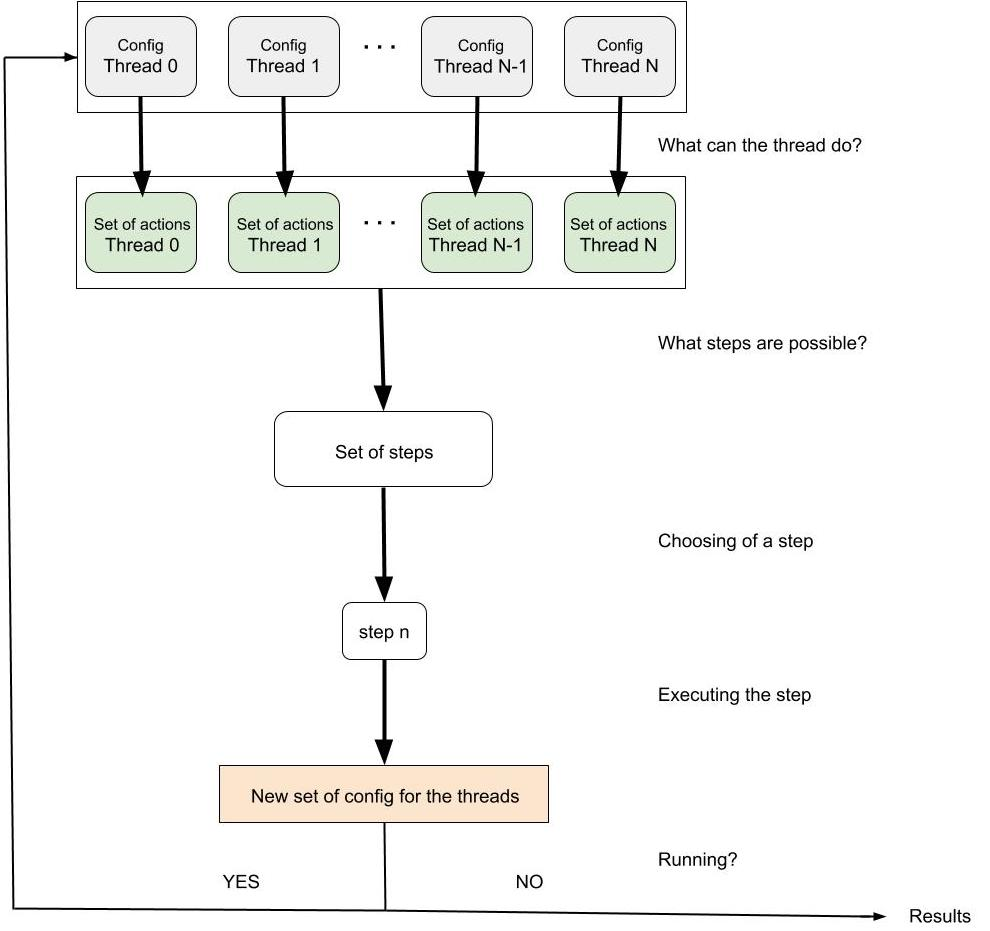
\includegraphics[scale = 0.4]{Interpretor_loop.jpg}
\caption{Interpretor loop}
\end{figure}

\newpage

\phantomsection
\addcontentsline{toc}{subsection}{Collection of the actions}
\tabto{1cm} {\Large \textsc{Collection of the actions}}
\vspace*{10pt}
\tabto{1cm}The first stage is to collect all the possible actions for each thread. There are five types of actions: tau, send, receive, spawn and beta actions. This last action corresponds to any of the beta reductions. Each thread can have a single possible action or a list of actions if the instruction for the thread is a choose.
\\ \\
\tabto{1cm}The communication actions - send and receive - contain an integer which is the identifier of the communication channel. When an action is found, it is coupled with the identifier of the thread and added to a list. So, for a thread we obtain a list of at least one couple. The list of all the actions is obtained by concatenating the list of all the threads.

\vspace*{10pt}
\vspace*{10pt}
\phantomsection
\addcontentsline{toc}{subsection}{Collection of the steps}
\tabto{1cm} {\Large \textsc{Collection of the steps}}
\vspace*{10pt}

\tabto{1cm}The next stage is to collect all the possible steps. There are four kind of steps: the tau, spawn, beta and communication steps. The last one contains the identifier of the channel, the sender and the receiver whereas the other steps just have the identifier of the thread on which they have to be executed. 
\\ \\
\tabto{1cm}To find the steps, we browse trough the list of actions. When the compiler finds an action that is not a communication actions, it converts the action into a step and add it to a list. For the communication actions, it adds the identifier of the thread and channel to a list of senders or receivers. When all actions have been analyzed, the compiler tries to find all the communication couples by matching each sender to all the possible receivers (the channel of the sender and receiver have to be identical).

\vspace*{10pt}
\vspace*{10pt}
\phantomsection
\addcontentsline{toc}{subsection}{Choice of the step}
\tabto{1cm} {\Large \textsc{Choice of the step}}
\vspace*{10pt}

\tabto{1cm}After collecting all the possible steps, the compiler has to choose which one to execute. To do that, the compiler generates a positive integer thanks to random number generator. So the index of the chosen step in the list is the remainder of the division of the number by the size of the list. Finally, the compiler retrieve the step by extracting it from the list of all the possible steps.

\vspace*{10pt}
\vspace*{10pt}
\phantomsection
\addcontentsline{toc}{subsection}{Execution of the step}
\tabto{1cm} {\Large \textsc{Execution of the step}}
\vspace*{10pt}

\tabto{1cm}To execute the step, the interpretor matches the step with the corresponding rule. In the case of a spawn step, it will retrieve a new configuration from the rule execution and add this configuration as a new thread. For the communication step, the compiler will first execute the send rule which returns the sent value and then run the receive rule which takes this value in argument. Finally, it is important to know that a beta step on a thread will in fact execute several beta steps. Indeed, the interpretor tries to run the maximum of beta steps when this type of steps is selected for a thread.  

\vspace*{10pt}
\vspace*{10pt}
\phantomsection
\addcontentsline{toc}{subsection}{Decision to loop or not}
\tabto{1cm} {\Large \textsc{Decision to loop or not}}
\vspace*{10pt}

\tabto{1cm}The execution of a step returns a status. This status can be two things "Running" or "Executed". The first one means that the compiler has found at least one step and has executed it. In this case, the interpretor will loop again at the first stage because it may have more steps to run. The second status means that the compiler has found no possible steps and so run nothing. In this case, the flow of execution is deadlock or finished, so the compiler returns the results. 

\vspace*{10pt}
\vspace*{10pt}
\phantomsection
\addcontentsline{toc}{section}{Technical notes}
\tabto{0cm}{\textbf{\LARGE Technical notes}}
\vspace*{3pt}
\vspace*{10pt}

\phantomsection
\addcontentsline{toc}{subsection}{Local and global variables}
\tabto{1cm} {\Large \textsc{Local and global variables}}
\vspace*{10pt}

\tabto{1cm}The programming language allows the declaration of global and local variables. However they are treated and initialized in a different way. The global variables have to be initialized when they are declared and cannot be modified after that. This choice has been made to avoid consideration on how to modify the global state.
\\ \\
\tabto{1cm} The local variables have to be declared in the "def" part of a function and can be used after in the "in" part. In fact, they do not need to be initialize even though not initializing the local variables is not a good practice. When the compiler calls a function, it immediately creates a new local state. This state contains the function parameters initialized  with expression passed as argument. Those parameters can be used like local variables inside the function. This new state also contains the local variable declarations. However those variables - having no initialization in the "def" part - are initialized to a default value depending on the type of the variable.

\vspace*{10pt}
\vspace*{10pt}
\phantomsection
\addcontentsline{toc}{subsection}{Garbage collector}
\tabto{1cm} {\Large \textsc{Garbage collector}}
\vspace*{10pt}

\tabto{1cm}To optimized the execution of a program, the compiler uses a garbage collector. This garbage collector detects the finished thread that do not return a value or return a void. This detection takes place when the compiler searches for the possible actions. When the thread is detected, the compiler immediately deletes its configuration from the hash table representing the threads. This allows the system to run faster because it is not hindered by useful threads. 
\\ \\
\tabto{1cm}This detection relies on the "Terminated" instruction. This instruction is set as the next instruction of the thread when its execution is complete, it can contain the final expression return by the thread if there is one. So the garbage collector will only delete dead threads - where the next instruction is "Terminated" without return - and not active or waiting threads.

\newpage

\phantomsection
\addcontentsline{toc}{section}{Semantic Rules}
\tabto{0cm}{\textbf{\LARGE Semantic Rules}}
\vspace*{3pt}
\vspace*{10pt}
\vspace*{10pt}

\phantomsection
\addcontentsline{toc}{subsection}{Semantic rules for expressions}
\tabto{1cm} {\Large \textsc{Semantics rules for expressions}}
\vspace*{20pt}

\tabto{0cm} {\large \textbf{Binary Operator}}
\begin{prooftree}
\AxiomC{$G;S \vdash e_1 \Downarrow  v_1 $}
\AxiomC{$G;S \vdash e_2 \Downarrow  v_2$}
\BinaryInfC{$G;S \vdash e_1 \ op \ e_2 \Downarrow v_1 \ op \ v_2 $}
\end{prooftree}

\tabto{0cm} {\large \textbf{Unary Operator}}
\begin{prooftree}
\AxiomC{$G;S \vdash e \Downarrow  v $}
\UnaryInfC{$G;S \vdash op \ e \Downarrow v $}
\end{prooftree}

\tabto{0cm} {\large \textbf{Condition Expression}}
\begin{prooftree}
\AxiomC{$G;S \vdash e_1 \Downarrow true $}
\AxiomC{$G;S \vdash e_2 \Downarrow v $}
\BinaryInfC{$G;S \vdash if \ e_1 \ then \ e_2 \ else \ e_3  \Downarrow v $}
\end{prooftree}
\vspace*{1pt}
\begin{prooftree}
\AxiomC{$G;S \vdash e_1 \Downarrow false $}
\AxiomC{$G;S \vdash e_3 \Downarrow v $}
\BinaryInfC{$G;S \vdash if \ e_1 \ then \ e_2 \ else \ e_3  \Downarrow v $}
\end{prooftree}


\tabto{0cm} {\large \textbf{Tuple}}
\begin{prooftree}
\AxiomC{$G;S \vdash e_1 \Downarrow v_1 $}
\AxiomC{$G;S \vdash e_2 \Downarrow v_2 $}
\AxiomC{$\ldots$}
\AxiomC{$G;S \vdash e_n \Downarrow v_n $}
\QuaternaryInfC{$G;S \vdash (e_1,e_2,\ldots,e_n) \Downarrow (v_1, v_2, \ldots, v_n)$}
\end{prooftree}

\tabto{0cm} {\large \textbf{Value}}
\begin{prooftree}
\AxiomC{ }
\UnaryInfC{$G;S \vdash v \Downarrow v $}
\end{prooftree}

\tabto{0cm} {\large \textbf{Identifier}}
\begin{prooftree}
\AxiomC{ }
\UnaryInfC{$G;S \vdash n \Downarrow lookup \ n \ in \ S $}
\end{prooftree}

\newpage

\phantomsection
\addcontentsline{toc}{subsection}{Semantic rules for instructions}
\tabto{1cm} {\Large \textsc{Semantics rules for instructions}}
\vspace*{20pt}

\tabto{0cm} {\large \textbf{Assignment}}
\begin{prooftree}
\AxiomC{$G;S \vdash e \Downarrow v $}
\UnaryInfC{$G;S;E \vdash a = e \rightarrow_{\beta} G;S::[a \mapsto v];E \vdash noop$}
\end{prooftree}

\tabto{0cm} {\large \textbf{Condition Instruction}}
\begin{prooftree}
\AxiomC{$G;S \vdash e \Downarrow true $}
\UnaryInfC{$G;S;E \vdash  if \ e \ then \ i_1 \ else \ i_2 \rightarrow_{\beta} G;S;E \vdash i_1$}
\end{prooftree}
\vspace*{1pt}
\begin{prooftree}
\AxiomC{$G;S \vdash e \Downarrow false $}
\UnaryInfC{$G;S;E \vdash  if \ e \ then \ i_1 \ else \ i_2 \rightarrow_{\beta} G;S;E \vdash i_2$}
\end{prooftree}

\tabto{0cm} {\large \textbf{Function Call with return}}
\begin{prooftree}
\AxiomC{$G;S \vdash \overrightarrow{e} \Downarrow \overrightarrow{v}$}
\AxiomC{$ G(f) = (\lambda \overrightarrow{x}.i,S_f)$}
\BinaryInfC{$G;S;E \vdash a = f (\overrightarrow{e}) \rightarrow_{\beta} G;G::[\overrightarrow{x} \mapsto \overrightarrow{v}]::S_f;(S;a=[.])::E \vdash i$}
\end{prooftree}

\tabto{0cm} {\large \textbf{Function Call without return}}
\begin{prooftree}
\AxiomC{$G;S \vdash \overrightarrow{e} \Downarrow \overrightarrow{v}$}
\AxiomC{$ G(f) = (\lambda \overrightarrow{x}.i,S_f)$}
\BinaryInfC{$G;S;E \vdash f (\overrightarrow{e}) \rightarrow_{\beta} G;G::[\overrightarrow{x} \mapsto \overrightarrow{v}]::S_f;(S;void)::E \vdash i$}
\end{prooftree}

\tabto{0cm} {\large \textbf{While Instruction}}
\begin{prooftree}
\AxiomC{$G;S \vdash e \Downarrow true $}
\UnaryInfC{$G;S;E \vdash  while(e) \ \{i\} \rightarrow_{\beta} G;S;E \vdash i; while(e) \ \{i\}$}
\end{prooftree}
\vspace*{1pt}
\begin{prooftree}
\AxiomC{$G;S \vdash e \Downarrow false $}
\UnaryInfC{$G;S;E \vdash  while(e) \ \{i\} \rightarrow_{\beta} G;S;E \vdash noop$}
\end{prooftree}

\tabto{0cm} {\large \textbf{Return void}}
\begin{prooftree}
\AxiomC{$ $}
\UnaryInfC{$G;S;(S';void)::E \vdash return \rightarrow_{\beta} G;S';E \vdash noop$}
\end{prooftree}


\tabto{0cm} {\large \textbf{Assign of a function return}}
\begin{prooftree}
\AxiomC{$ $}
\UnaryInfC{$G;S;(S';a=[.])::E \vdash return \ v \rightarrow_{\beta} G;S';[a \mapsto v]::E \vdash noop$}
\end{prooftree}

\tabto{0cm} {\large \textbf{Return Break}}
\begin{prooftree}
\AxiomC{$ $}
\UnaryInfC{$G;S;(seqi)::E \vdash return \ e \rightarrow_{\beta} G;S;E \vdash return \ e$}
\end{prooftree}

\tabto{0cm} {\large \textbf{Sequence of Instructions}}
\begin{prooftree}
\AxiomC{$ $}
\UnaryInfC{$G;S;E \vdash i ; seqi \rightarrow_{\beta} G;S;(seqi)::E \vdash i$}
\end{prooftree}

\tabto{0cm} {\large \textbf{Noop}}
\begin{prooftree}
\AxiomC{$ $}
\UnaryInfC{$G;S;(seqi)::E \vdash noop \rightarrow_{\beta} G;S;E \vdash seqi$}
\end{prooftree}

\tabto{0cm} $\Delta = G;S;E$

\tabto{0cm} {\large \textbf{NewChan Instruction}}
\begin{prooftree}
\AxiomC{$ $}
\UnaryInfC{$ N;\Delta \vdash a = newChan() \rightarrow_{\beta} N \oplus {n};\Delta[a \mapsto n] \vdash noop $}
\end{prooftree}

\tabto{0cm} {\large \textbf{Receive Instruction}}
\begin{prooftree}
\AxiomC{$N;S \vdash ch \Downarrow n$}
\UnaryInfC{$N;\Delta \vdash a = receive(ch) \underset{n?v}{\longrightarrow} N;\Delta[a \mapsto v] \vdash noop $}
\end{prooftree}

\tabto{0cm} {\large \textbf{Send Instruction}}
\begin{prooftree}
\AxiomC{$N;S \vdash ch \Downarrow n$}
\AxiomC{$N;S \vdash e \Downarrow v$}
\BinaryInfC{$N;\Delta \vdash send(ch,e) \underset{n!v}{\longrightarrow} N;\Delta \vdash noop$}
\end{prooftree}

\tabto{0cm} {\large \textbf{Choose Instruction}}
\begin{prooftree}
\AxiomC{$ $}
\UnaryInfC{$N;\Delta \vdash choose \{ \overrightarrow{ \ p \longrightarrow i \ } \} \rightarrow N;G;S;(i_k)::E \vdash p_k $}
\end{prooftree}

\tabto{0cm} {\large \textbf{Spawn Instruction}}
\begin{prooftree}
\AxiomC{$G;S \vdash \overrightarrow{e} \Downarrow \overrightarrow{v}$}
\AxiomC{$ G(f) = (\lambda \overrightarrow{x}.i,S_f)$}
\BinaryInfC{$\Delta \vdash spawn f (\overrightarrow{e})
 \xrightarrow[\text{ spawn(G;S; . ) $\vdash$ i}]{} \Delta \vdash noop$}
\end{prooftree}

\newpage

\phantomsection
\addcontentsline{toc}{chapter}{Examples}
\label{Examples}
\centerline{\textbf{\Huge Examples}}

\vspace*{15pt}

\centerline{Presentation of the different examples present in the examples folder of the package examples.}
\vspace*{5pt}
\tabto{0cm}{The first 3 examples are from the book \textit{Communicating and mobile systems: the $\pi$-calculus} by Robin Milner }

\phantomsection
\addcontentsline{toc}{section}{Mobiles phones (example-00)}
\tabto{0cm}{\textbf{\LARGE Mobiles phones (example-00)}}
\vspace*{3pt}
\vspace*{20pt}
\\
\tabto{0cm}{This example is highly inspired by the "mobile phones system" example - page 82.}
\vspace*{3pt}
\vspace*{10pt}
\begin{center}
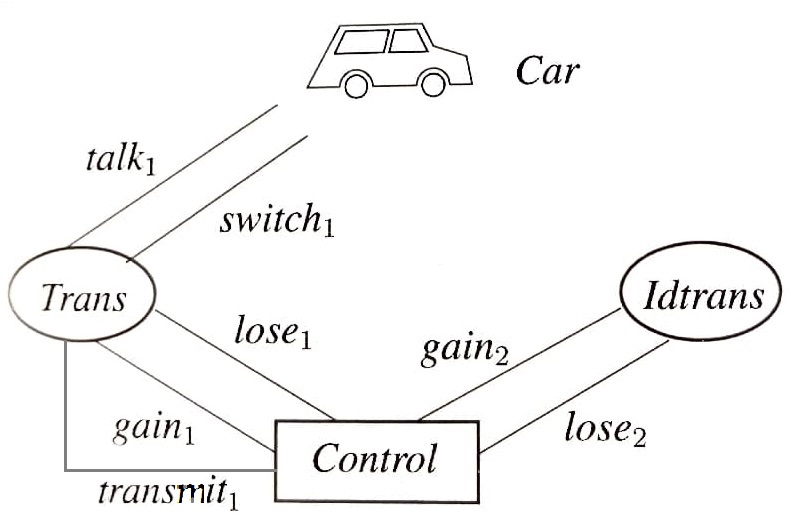
\includegraphics[scale = 0.7]{mobile-phone-system.jpg}
\end{center}
\vspace*{3pt}
\vspace*{10pt}

\tabto{0cm}{In our example, we made some modifications compared to the original example from the book. To allow the control to know when it needs to act we add an other channel between Control and Trans named transmit1. This channel transmits the message received by Trans from Car. This message is an integer which represents the position of the car. We arbitrarily decide at which position the links between the Trans and the car must be switched to the other trans : Idtrans. So, when the position is greater than the threshold the Control tells to Trans to lose the car and to IdTrans to gain the car.}
\newpage

\vspace*{15pt}
\phantomsection
\addcontentsline{toc}{section}{Buffer of size n (example-01)}
\tabto{0cm} {\LARGE \textbf{Buffer of size n (example-01)}}
\vspace*{3pt}
\vspace*{10pt}
\\
\tabto{1cm}{This example is highly inspired by the "Buffer of size n" example - page 84.} \\ \\
In this example, we consider a buffer of n cells. First, in $\pi$-calculus the definition of a buffer cell is :
$B(l,r) = l(x).C \langle x,l,r \rangle$ and $C(x,l,r) = \bar{r} \langle x \rangle .B \langle l,r \rangle$
\vspace*{3pt}
\vspace*{10pt}
\begin{center}
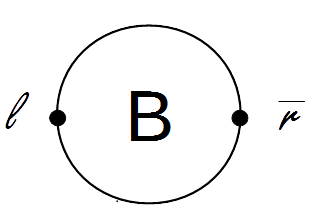
\includegraphics[scale = 0.5]{BufferCell.png}
\end{center}
So to create a buffer of size n, we make a chain of n buffer cells. This system is defined by linking :
$B^{(n)} = \overbrace{B^{ \frown} \ldots ^{\frown} B}^{\text{n times}}$
\vspace*{3pt}
\vspace*{10pt}
\begin{center}
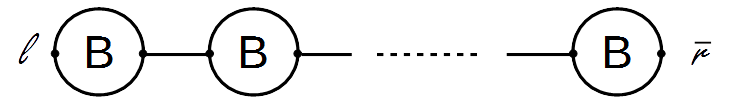
\includegraphics[scale = 0.6]{Buffern.png}
\end{center}

\phantomsection
\addcontentsline{toc}{section}{Condition with channels (example-02)}
\tabto{0cm} {\LARGE \textbf{Condition with channels (example-02)}} \\
\vspace*{3pt}
\\
\tabto{1cm}{This example is highly inspired by the "Condition with channels" example - page 104.} \\ \\
In this example, we use a condition of type \textit{if then else} based on channels. First, we created the true and false value thanks to channels. We can defined those values in $\pi$-calculus : \\ \\
\centerline{$True(l) = l(t,f). \bar{t}$ \ and \ $False(l) = l(t,f). \bar{f}$} \\
\\ Then we can create a condition by using those values.
The condition needs a channel l which corresponds to the location of a value true or false. It is defined as follow : \\ \\
\centerline{$ Cond(P,Q)(l) = (new (t,f)) \bar{l} \langle t,f \rangle .(t.P + f.Q)$} \\
\\Depending on that the condition process will launch a different process. The processes P and Q are represented in our grammar by function which has to be spawned by the process condition. 

\phantomsection
\addcontentsline{toc}{section}{Chemical reaction (example-03)}
\tabto{0cm} {\LARGE \textbf{Chemical reaction (example-03)}}
\vspace*{3pt}
\vspace*{10pt}

\tabto{1cm}{This example is highly inspired by the "KNa2Cl" example - slide 14  from the course \textit{On pi-Calculus and its Applications} by Luca Gardelli } \\ \\
In this example we are trying to simulate the following chemical reaction : \\
$K + Na + 2Cl = K^+ + Na^+ + 2Cl^-$ \\
For each type of atoms, there are dedicated channels on which they liberate or capture an electron. The ionization and deionization process are associated with the receive and send instructions. An atom can capture an electron only if an another atom is ready to liberate one and vice-versa. In our example, the thermochemical laws are not respected because the reaction can occur in both ways at anytime.  

\begin{figure}[!h]
    \centering
    \begin{subfigure}[b]{0.3\textwidth}
        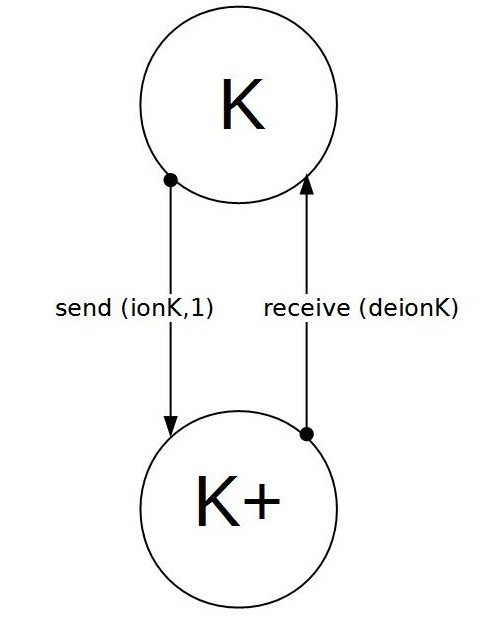
\includegraphics[width=\textwidth]{K.jpg}
    \end{subfigure}
    \begin{subfigure}[b]{0.3\textwidth}
        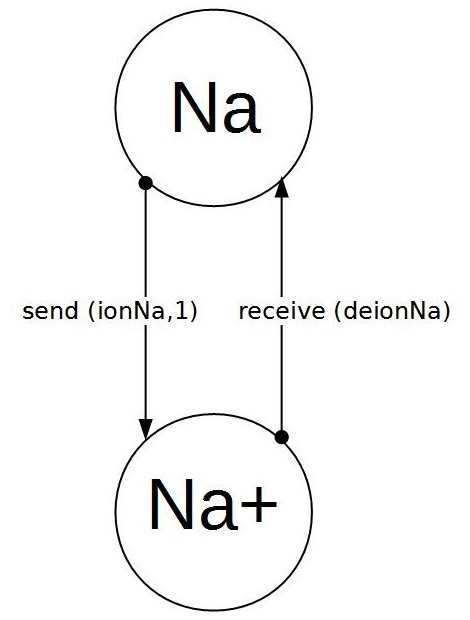
\includegraphics[width=\textwidth]{Na.jpg}
    \end{subfigure}
    \begin{subfigure}[b]{0.3\textwidth}
        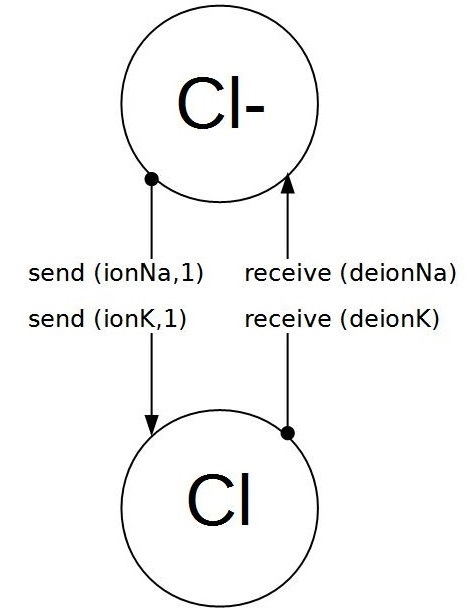
\includegraphics[width=\textwidth]{Cl.jpg}
    \end{subfigure}
\end{figure}

\phantomsection
\addcontentsline{toc}{section}{Dining philosophers problem (example-04)}
\tabto{0cm} {\LARGE \textbf{Dining philosophers problem (example-04)}}
\vspace*{3pt}
\vspace*{10pt}
\tabto{1cm}In this example, we have chosen to represent the dining philosophers problem, a recurring concurrent problem.
\begin{center}
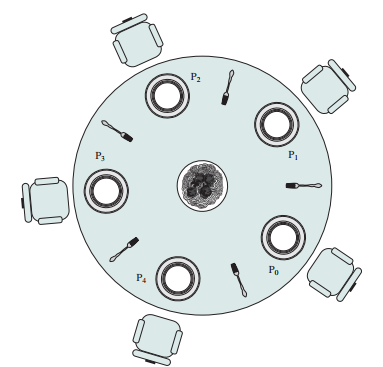
\includegraphics[scale = 0.55]{Dining.png}
\end{center}

\tabto{0cm}N philosophers sit at a round table with meal plates. Forks are placed between each pair of adjacent philosophers.
\\ Each philosopher must alternately think and eat. However, a philosopher can only eat the meal when they have both left and right forks. Each fork can be held by only one philosopher and so a philosopher can use the fork only if it is not being used by another philosopher. After an individual philosopher finishes eating, they need to put down both forks so that the forks become available to others. A philosopher can take the fork on their right or the one on their left as they become available, but cannot start eating before getting both forks.
\\ \\
\phantomsection
\addcontentsline{toc}{section}{Whispering problem (example-05)}
\tabto{0cm} {\LARGE \textbf{Whispering problem (example-05)}}
\vspace*{3pt}
\vspace*{10pt}
\tabto{1cm}{This example is highly inspired by the "The Rumor Mill at the Hannenfass bar" example by Thomas Schneider}

\tabto{0cm}In this example, we have represented a situation in a bar. In this one there is a barman, customers who don't know the secret and a customer who knows the secret (There is only one secret). The barman can install 2 people at a table.  One of the 2 people will speak first, the other will listen and then both will leave the table. So, several situations are possible:
\begin{itemize}
    \item the 2 people don't know the secret: they discuss and leave the table without knowing the secret. \\
    \item  one of the 2 people knows the secret and the wise man speaks first: He's going to tell this secret or not to the second person. If he reveals the secret to the second person, this person now knows it and can spread it to other customers, if he does not reveal it the person who did not know the secret still does not know it when he leaves the table.   \\
    \item one of the 2 people knows the secret but the wise man doesn't speak first: the person who did not know the secret still does not know it when he leaves the table. \\
    \item the 2 people know the secret: The situation will not change, they leave the table knowing the secret.
\end{itemize}
The secret can be transmitted and spread throughout the bar.
\end{document}
